\documentclass[notes]{beamer}


\usepackage{amsfonts}
\usepackage{amssymb}
\usepackage{amsthm}

\mode<presentation>
{
  \usetheme{default}      % or try Darmstadt, Madrid, Warsaw, ...
  \usecolortheme{default} % or try albatross, beaver, crane, ...
  \usefonttheme{default}  % or try serif, structurebold, ...
  \setbeamertemplate{navigation symbols}{}
  \setbeamertemplate{caption}[numbered]
} 

\usepackage[english]{babel}
\usepackage[utf8]{inputenc}
\usepackage[T1]{fontenc}
\newcommand{\fancy}[1]{\mathcal{#1}}

\newcommand{\thepicone}{
\includegraphics[width=5cm,height=5cm,keepaspectratio]{news_clip1.png}}

\newcommand{\thepictwo}{
\includegraphics[width=5cm,height=5cm,keepaspectratio]{news_clip2.png}}

\newcommand{\thepicthree}{
\includegraphics[width=5cm,height=5cm,keepaspectratio]{news_clip3.png}}

\newcommand{\thepicfour}{
\includegraphics[width=5cm,height=5cm,keepaspectratio]{news_clip4.png}}

\newcommand{\thepicfive}{
\includegraphics[width=5cm,height=5cm,keepaspectratio]{news_clip5.png}}

\newcommand{\thepicsix}{
\includegraphics[width=5cm,height=5cm,keepaspectratio]{news_clip6.png}}

\begin{document}






\begin{frame}{Motivation}

\thepicone
\alt<2->{\thepictwo}{\phantom{\thepictwo}}
\alt<3->{\thepicthree}{\phantom{\thepicthree}}
\alt<4->{\thepicfour}{\phantom{\thepicfour}}
\alt<5->{\thepicfive}{\phantom{\thepicfive}}
\alt<6->{\thepicsix}{\phantom{\thepicsix}}


\end{frame}







\begin{frame}{Motivation}



\begin{itemize}
 \item<1-> In the U.S. there are 297 million insured, 87 million underinsured, 27 million uninsured
 \item<2-> What role does the uninsured/underinsured population play in the progress of a pandemic? 
 \item<3-> When to implement universal insurance coverage and how quickly?
 
\end{itemize}






\end{frame}


\begin{frame}{Key Measures}

\begin{itemize}
  \item Peak ICU Hospitalization
    \item Average ICU Hospitalization
    \item Total Deaths
\end{itemize}

Other measures that could be interesting:
\begin{itemize}
    \item Days over/under ICU capacity
    \item Peak Infections
\end{itemize}

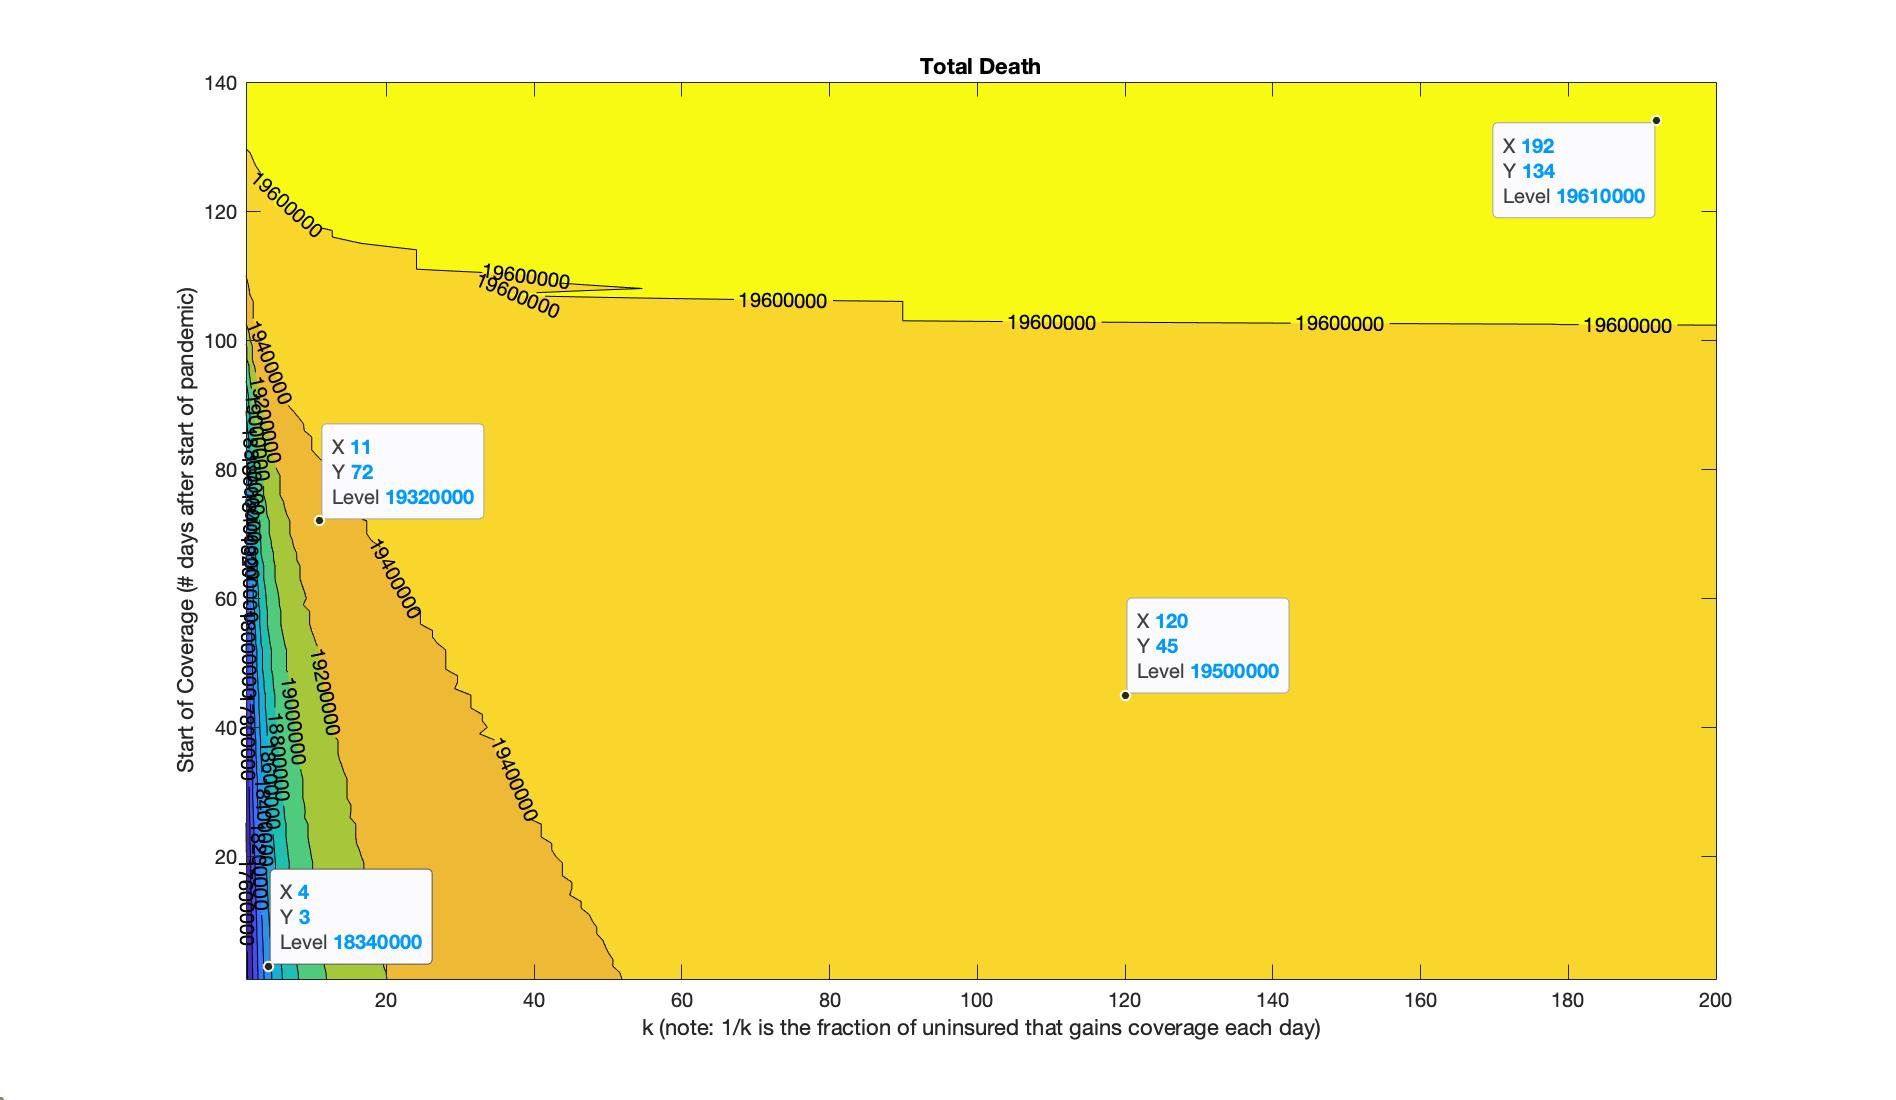
\includegraphics[width=10cm,height=10cm,keepaspectratio]{run.jpg}

\end{frame}

\begin{frame}{Which mathematical tools can answer this question?}



% Before we proceed I want to note that this is still very much a work in progress.  So I would like feedback whenever possible.



\end{frame}


\begin{frame}{SIHR model}


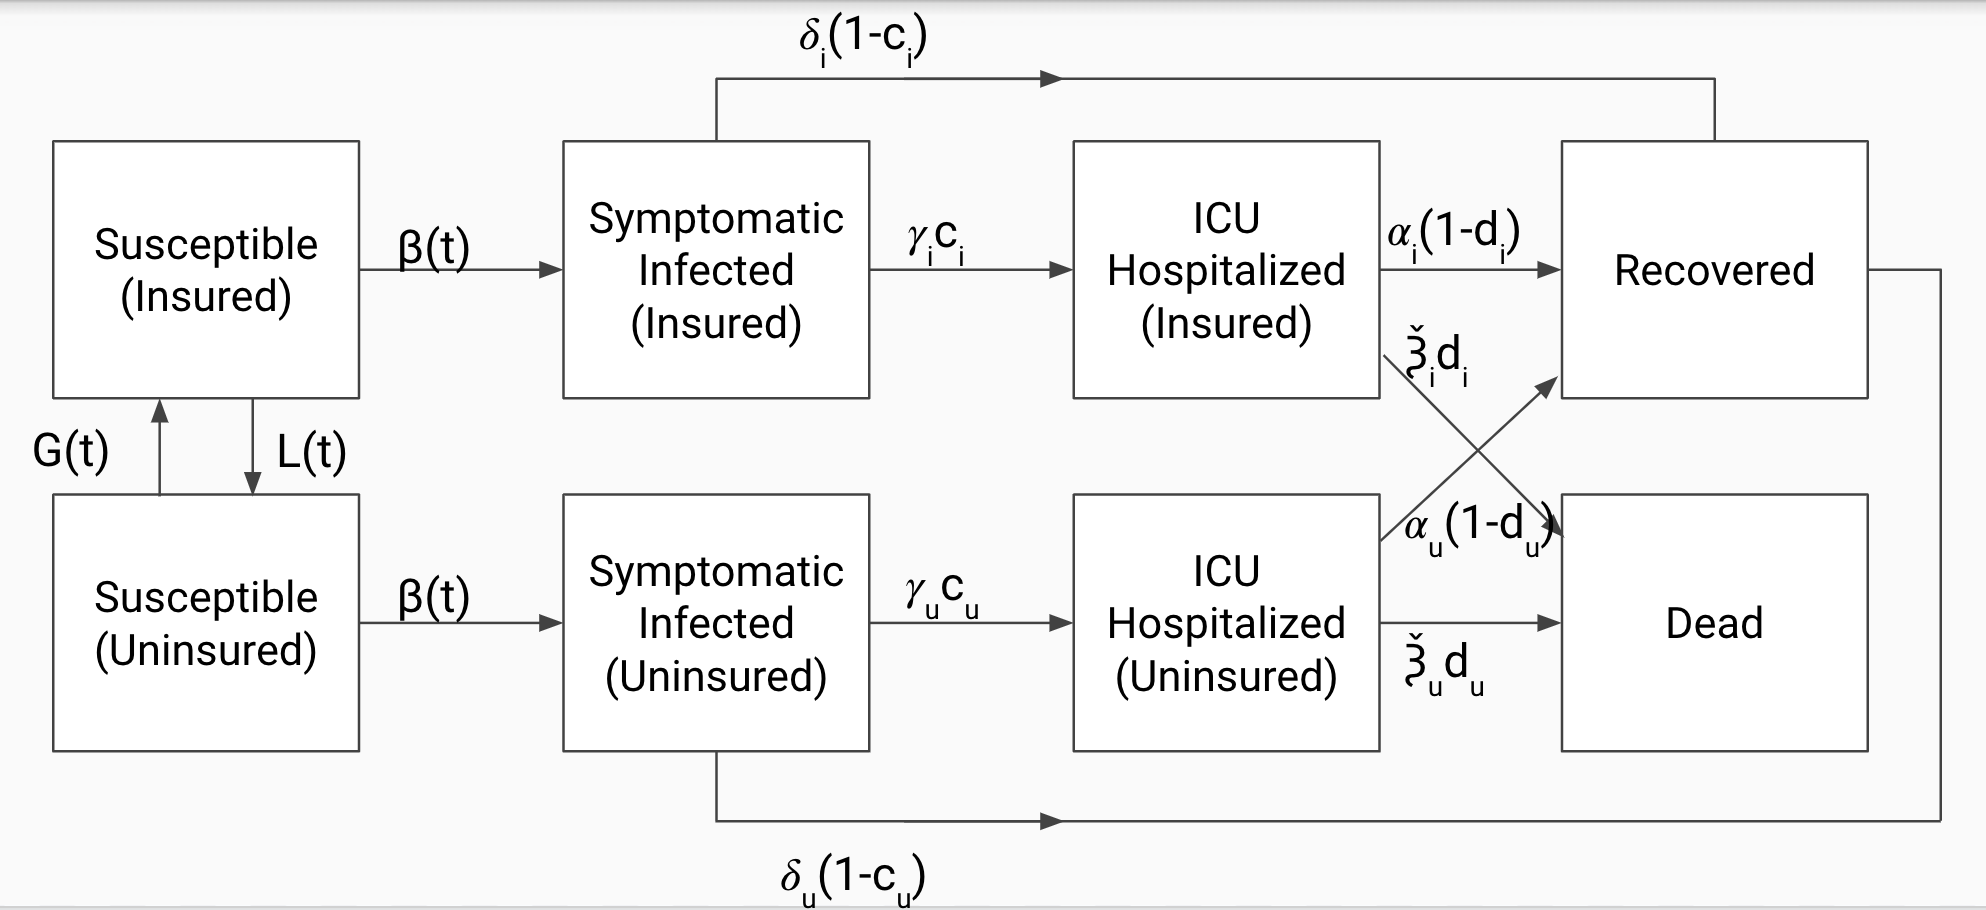
\includegraphics[width=12cm,height=12cm,keepaspectratio]{model_flow.png}






\end{frame}

\begin{frame}[shrink=25]{Parameters}

\begin{tabular}{|c|c|c|c|}
    \hline
    \textbf{parameter} & \textbf{description} & \textbf{value} & \textbf{units} \\
    \hline
    $S_{u,0}$ & Susceptible uninsured population & 27.5 million & \# people\\
    \hline
    $S_{u,0}$ & Susceptible under-insured population & 87 million & \# people\\
    \hline
    $S_{i,0}$ & Susceptible insured population & 296 million & \# people\\
    \hline
    $h$ & Probability that symptomatic infected go to ICU & 0.05 & fraction \\
    \hline
    $c_{i}$ & Probability that insured symp. infec. go to ICU & 0.045 & fraction \\
    \hline
    $c_{u}$ & Probability that insured symp. infec. go to ICU & 0.107 & fraction \\
    \hline
    $k$ & Probability that ICU patient will die & 0.236 & fraction \\
    \hline
    $d_{i}$ & Probability that insured ICU patient will die & 0.225 & fraction\\
    \hline
    $d_{u}$ & Probability that uninsured ICU patient will die & 0.283 & fraction \\
    \hline
    $\gamma_{i,u}$ & Rate at which those infected go to ICU & $1/5$ & 1/days \\
    \hline
   $\delta_{i,u}$ & Rate at which infected recovery & $1/14$ & 1/days\\
    \hline
    $\beta$ & Contact rate/infection probability & 0.5 & 1/days \\
    \hline
    $\xi_{i,u}$ & Death rate & $1/3$ & 1/days \\
    \hline
    $\alpha_{i,u}$ & Rate at which ICU hospitalization recovers & $1/14$ & 1/days\\
    \hline
    $L(t)$ & loss-of-coverage & - & 1/days  \\
    \hline
    $G(t)$ & gain-of-coverage & - & 1/days \\
    \hline
      $t_s$ & universal coverage start time & - & days \\

    \hline
    \end{tabular}

\end{frame}

\begin{frame}[shrink=25]{Assumptions and Simplifications}
%Below are some assumptions and caveats that stood out to me




\begin{itemize}
    \item<1-> People in ICU do not infect others
    \item<2-> Uninsured people are more likely (than insured people, of course) to require ICU hospitalization due to possible mismanagement of comorbidities and delays in seeking non-emergency care ($c_u > c_i$).
\item<3-> Uninsured people are more likely to die once in ICU hospitalization ($d_u > d_i$).
 \item<4-> The rate at which ICU hospitalization recovers is equal for insured and uninsured.
\item<5-> Contact rates are the same for uninsured and insured populations
\item<6-> Increase in monthly unemployment fraction means a proportional transfer of people from the susceptible insured compartment to the susceptible uninsured compartment
\item<7-> Once an insured person loses insurance coverage, there is a delay before they begin to “act” like an uninsured person, from the perspective of this model. That is, it take n days before the impacts of delay in seeking care and mismanagement of any comorbidities increase their chances of needing ICU hospitalization once infected.

\item<8-> There is long-lasting immunity 

    \item<9-> No one (i.e., not a significant number) dies from COVID-19 without first needing ICU hospitalization. 
\item<10-> Not important to track asymptomatic people to help answer our questions.

    
\end{itemize}


 

 

 
 
 
 





\end{frame}


\begin{frame}[shrink=25]{SIHR model}





$$\frac{dS_u(t)}{dt} = -\beta\left(\frac{I_i(t) + I_u(t)}{N}\right)S_u(t) + L(t) S_i(t) - G(t) S_u(t)$$

$$\frac{dS_i(t)}{dt} = -\beta\left(\frac{I_i(t) + I_u(t)}{N}\right)S_i(t) - L(t) S_i(t) +  G(t) S_u(t)$$

$$\frac{dI_u(t)}{dt} = \beta\left(\frac{I_i(t) + I_u(t)}{N}\right)S_u(t) - 
\gamma_u c_u I_u(t) - \delta_u (1-c_u) I_u(t)$$

$$\frac{dI_i(t)}{dt} = \beta\left(\frac{I_i(t) + I_u(t)}{N}\right)S_i(t) - 
\gamma_i c_i I_i(t) - \delta_i (1-c_i) I_i(t)$$

$$\frac{dH_u(t)}{dt} =   
\gamma_u c_u I_u(t) - \xi_u d_u H_u(t) - \alpha_u (1-d_u)H_u(t)$$

$$\frac{dH_i(t)}{dt} =   
\gamma_i c_i I_i(t) - \xi_i d_i H_i(t) - \alpha_i (1-d_i)H_i(t)$$

$$\frac{dR_u(t)}{dt} = \delta_u (1-c_u) I_u(t) + \alpha_u (1-d_u)H_u(t)$$

$$\frac{dR_i(t)}{dt} = \delta_i (1-c_i) I_i(t) + \alpha_i (1-d_i)H_i(t)$$

$$\frac{dD_u(t)}{dt} =  \xi_u d_u H_u(t)$$

$$\frac{dD_i(t)}{dt} = \xi_i d_i H_i(t)$$






\end{frame}



\begin{frame}{Loss of Coverage and time-varying $\beta$}



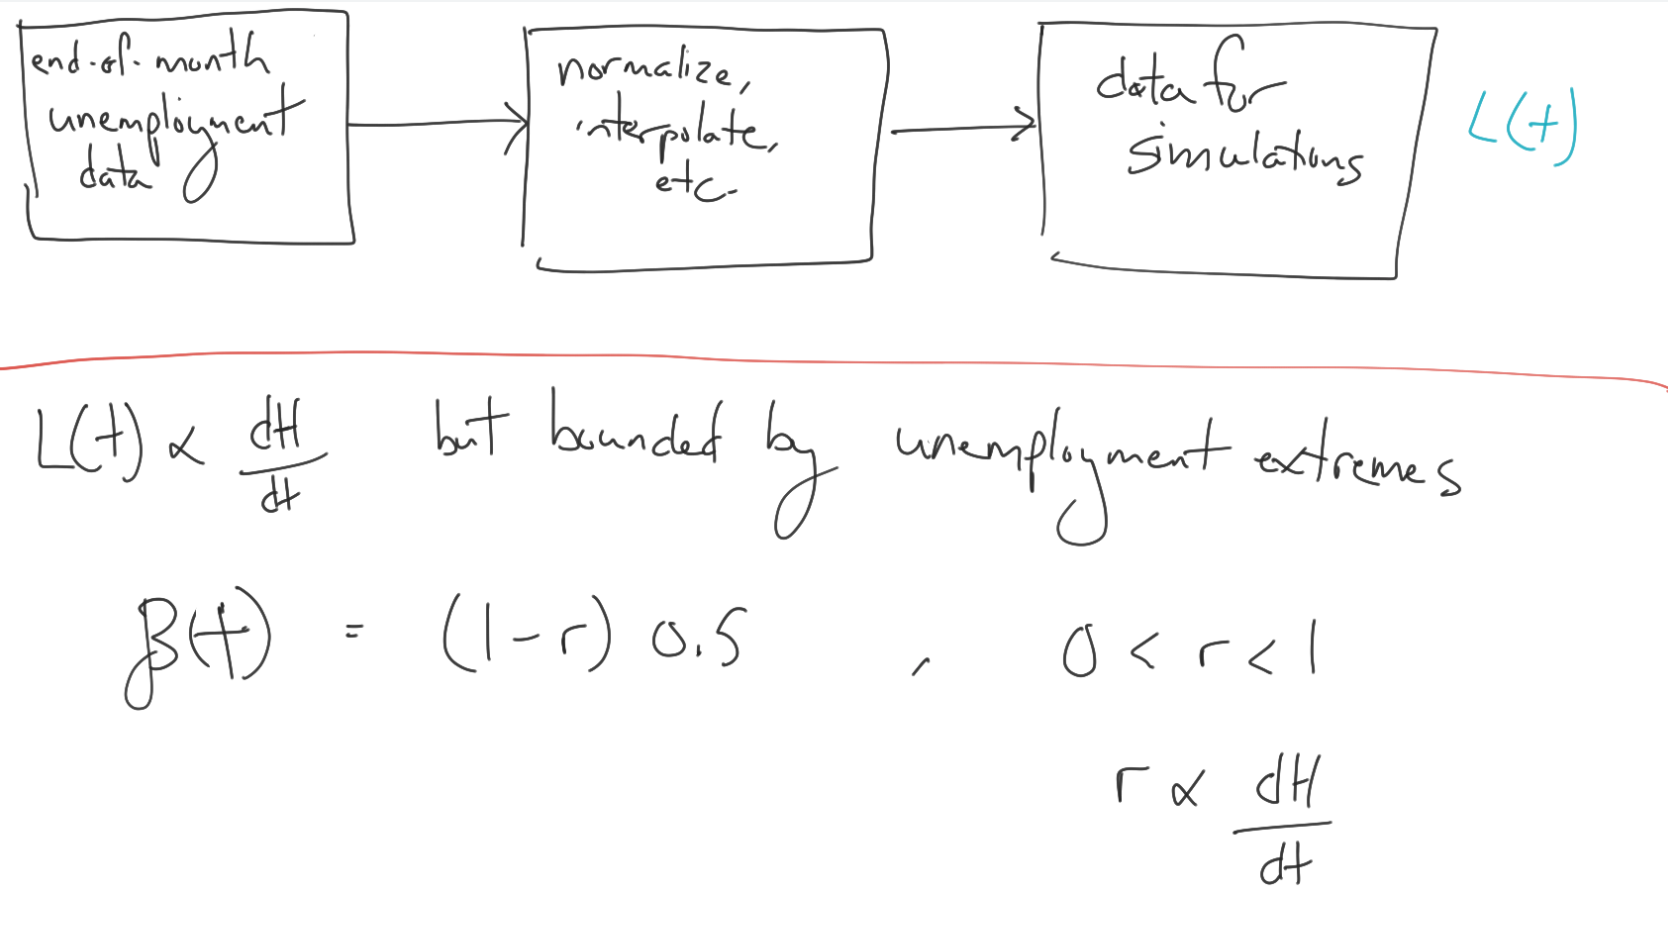
\includegraphics[width=10cm,height=10cm,keepaspectratio]{loss_and_beta.png}




\end{frame}




\begin{frame}{Gain of Coverage}



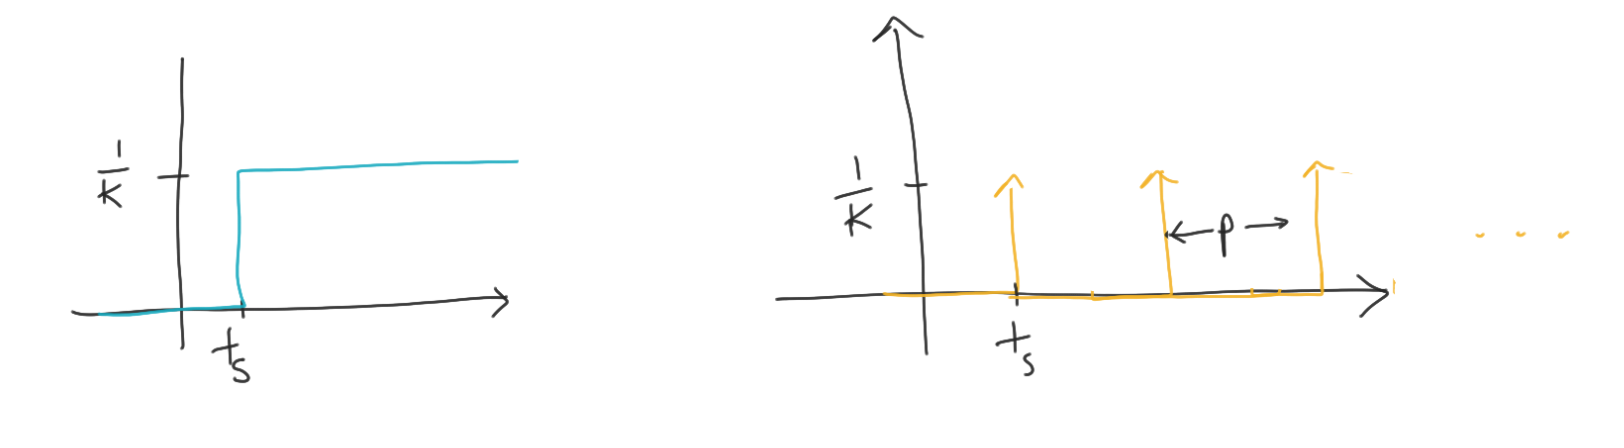
\includegraphics[width=10cm,height=10cm,keepaspectratio]{gain.png}

\end{frame}




\begin{frame}{Understanding the Model and Sensitivity to Parameters}


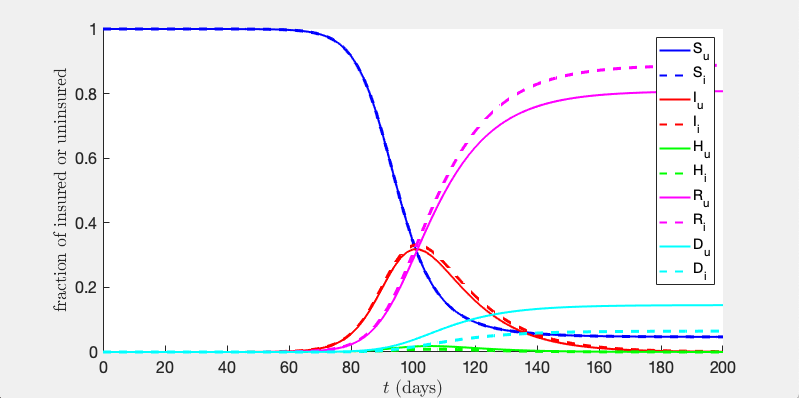
\includegraphics[width=10cm,height=10cm,keepaspectratio]{image1.png}




\end{frame}

\begin{frame}{Understanding the Model and Sensitivity to Parameters}

$$h = p_i\cdot c_i + p_u \cdot c_u$$

$$k = p_i\cdot d_i + p_u \cdot d_u$$



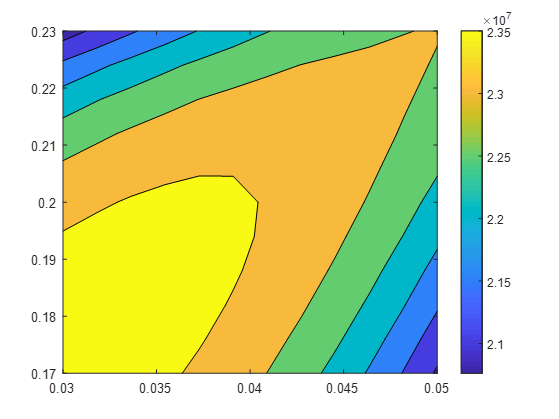
\includegraphics[width=8cm,height=8cm,keepaspectratio]{image11.png}


\end{frame}




\begin{frame}{Improvements to the Model}

\begin{itemize}
 \item<1-> Age structuring
 \item<2-> Cost of implementing universal coverage
 \item<3-> ICU rejecting patients
 
\end{itemize}


\end{frame}





\end{document}